\documentclass{article}  
\usepackage{tikz}
\usetikzlibrary{decorations.pathreplacing}
\usepackage{multicol}
\usepackage{amsmath}
\usepackage[a4paper]{geometry}
\usepackage{fancyhdr}
\pagestyle{fancy}
\lhead{Ableitungen}
\rhead{März 2025 - Juli 2025}
\begin{document} 
 
\newcommand{\derive}{\frac{\mathrm{d}}{\mathrm{d}x}}  
\newcommand{\bitem}[1]{\text{\textbf{#1}}} 
  
\section{Ableitungen}
\begin{minipage}{\dimexpr\linewidth-5cm} 
Die Ableitung $f'$ einer Funktion $f$ beschreibt ist eine Funktion, welche für jedes $x$ bei $f'(x)$ die Steigung am Punkt $f(x)$ angibt. Ähnlich wie bei linearen Funktionen kann die Steigung mit dem Steigungsdreieck, $m=\frac{\Delta y}{\Delta x}$ annähern, wenn $\Delta x$ zu null geht. Wird das $\Delta x$ durch $h$ dargestellt, ist offensichtlicherweise ${\Delta y = f(x+h)-f(x)}$, heißt es gilt an jedem Punkt $x$
\[
 f'(x) = \lim_{h \to 0} \frac{f(x+h)-f(x)}{h}
\]
\end{minipage}
\hfill
\begin{minipage}{5cm}
 \centering
 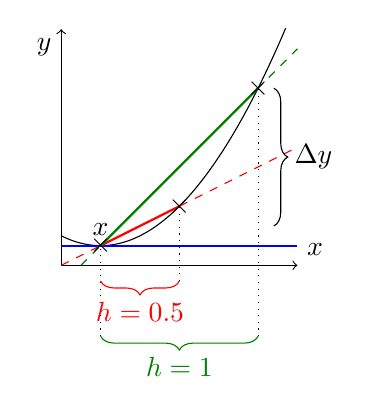
\begin{tikzpicture}
  \draw[domain=0:2.85, samples=75] 
   plot (\x, {0.5*(\x-0.5)^2+0.25});
  \draw[->] (0,0) -- (3,0) node [above right] {$x$};
  \draw[->] (0,0) -- (0,3) node [below left] {$y$};
    
  \draw[blue, thick] (0,0.25) -- (3, 0.25);
  \draw[red, dashed] (0,0) -- (3, 1.5);  
  \draw[red, thick] (0.5,0.25) -- (1.5, 0.75);
  \draw[green!50!black, dashed] (0.25,0) -- (3, 2.75); 
  \draw[green!50!black, thick] (0.5,0.25) -- (2.5, 2.25);
  
  \draw[dotted] (0.5,-0.9) -- (0.5, 0.25);  
  \draw[dotted] (1.5,-0.2) -- (1.5, 0.75); 
  \draw[dotted] (2.5,-0.9) -- (2.5, 2.25);
 
  \draw (0.5, 0.25) node {$\times$} node [above] {$x$};
  \draw (1.5,0.75) node {$\times$};
  \draw (2.5,2.25) node {$\times$};
  
  \draw [green!50!black, decorate,decoration={brace,amplitude=5pt,mirror}]
  (0.5,-0.9) -- (2.5,-0.9) node[midway,below,yshift=-4pt]{$h=1$};  
  \draw [red, decorate,decoration={brace,amplitude=5pt,mirror}]
  (0.5,-0.2) -- (1.5,-0.2) node[midway,below,yshift=-4pt]{$h=0.5$};
  \draw [decorate,decoration={brace,amplitude=5pt,mirror}]
  (2.7,0.5) -- (2.7,2.25) node[midway,right,xshift=4pt]{$\Delta y$};
 \end{tikzpicture} 
\end{minipage} 
 
\section{Ableitungsregeln}
$\mathrm{C}$ als Konstante 
\begin{multicols}{2} 
 \noindent \begin{align*}
  &\bitem{Summenregel} &&\derive (u + v) = u' + v' \\
  &\bitem{Faktorregel} &&\derive (\mathrm{C} \cdot u) = \mathrm{C} \cdot u' \\  
  &\bitem{Produktregel} &&\derive (u \cdot v) = u' \cdot v + v' \cdot u \\
  &\bitem{Quotientenregel} &&\derive \left( \frac{u}{v} \right) = \frac{u' \cdot v - v' \cdot u}{v^2} \\
 &\bitem{Kettenregel} &&\derive f(g(x)) = f'(g(x)) \cdot g'(x) \\
 \end{align*} 
 \begin{align*}
  &\bitem{e-Funktion} &&\derive \mathrm{e}^x = \mathrm{e}^x \\
  &\bitem{ln-Funktion} &&\derive \ln x = \frac{1}{x} \\
  &\bitem{sinus-Funktion} &&\derive \sin x = \cos x \\
  &\bitem{cosinus-Funktion} &&\derive \cos x = -\sin x
 \end{align*} 
\end{multicols} 
\end{document}
 
 
 
 
 
 
